% To make a PDF from this source, use the pdflatex command.
\documentclass[helvetica,english,utf8,notitle,nologo]{beamer}
\usetheme{default}
\usecolortheme{seahorse}
\usepackage{graphicx}
\graphicspath{ {images/} }

\begin{document}

\title{Intro to Docker}
\author{Carlos Konstanski}

\frame{\titlepage}

\begin{frame}
  \frametitle{Presentation Materials Available Online At:}
  \href{url}{https://github.com/ckonstanski/docker-presentation}
\end{frame}

\begin{frame}
  \frametitle{Supported Platforms}

  Docker runs on Linux, Mac OSX and Windows. 

  This presentation is done entirely on Linux. From a user interface
  standpoint things should be nearly identical on Mac and Windows
  (according to the Docker website).
\end{frame}

\begin{frame}
  \frametitle{What Is Virtualization?}

  To understand containerization, it is useful to examine how it
  differs from virtualization.

  Virtualization is when an entire operating system, consisting of
  both kernel and user space, runs inside a single process within
  another operating system. The parent OS provides software-emulated
  hardware for the virtualized OS.

  The emulated hardware might be implemented entirely in software, or
  it might be a thin software wrapper around real hardware.
\end{frame}

\begin{frame}
  \frametitle{What Is a Chroot Jail?}

  Another useful concept to understand as a prerequisite to
  containerization is the chroot jail.

  Every process has access to the filesystem. By default the
  filesystem that the process sees has its root at /. A chroot jail is
  a means of limiting the process' access to the filesystem by
  restricting its / to a subdirectory.

  Every filesystem resource that the chrooted process requires must be
  present inside the chroot directory tree. It will have its own
  /usr/bin, /usr/lib, /lib, /dev, /proc, etc. with copies of all
  needed executables, shared objects, etc.

  Examples of common programs that typically run in a chroot:

  \begin{itemize}
  \item bind
  
  \end{itemize}

  Demonstration: mount a Linux filesystem from a rescue CD and chroot
  into it.
\end{frame}

\begin{frame}
  \frametitle{What Is Containerization?}

  Containerization is something in between a chroot and a virtual
  machine, more closely resembling a chroot.

  There is no kernel space in a container, only userspace. Since the
  parent OS is providing the kernel space, there is no need for
  hardware emulation.

  The linux features that make containers possible are namespaces and
  cgroups.

  A quick read to familiarize yourself with the basics of namespaces
  and cgroups:

  https://jvns.ca/blog/2016/10/10/what-even-is-a-container/
\end{frame}

\begin{frame}
  \frametitle{What Is Docker?}

  Docker is a system that uses namespaces and cgroups at its core,
  plus some extra goodies on top, to provide a very easy to use
  containerization platform. Some of these goodies are:

  \begin{itemize}
  \item A registry where prebuilt containers can be stored
  \item A simple means to build containers with customizations
  \item Private networking for free
  \item A means to mount directories on the host filesystem
  \end{itemize}

  Other such platforms exist, for instance LXC. Docker is just the
  most popular.
\end{frame}

\begin{frame}
  \frametitle{Docker Registry}

  The Docker Registry is a storage and retrieval system for prebuilt
  Docker containers. You can either use the public registry, or you
  can set up your own private one. The public registry is called
  Docker Hub.
\end{frame}

\begin{frame}
  \frametitle{Docker Hub}

  Docker Hub is a public web service: https://hub.docker.com/explore/

  It contains lots of free prebuilt docker images. An image can be
  downloaded by using the docker pull command or by referenceing it in
  your Dockerfile.
\end{frame}

\begin{frame}
  \frametitle{Docker Pull}

  Example: using the docker pull command to download the latest Ubuntu
  LTS image.

  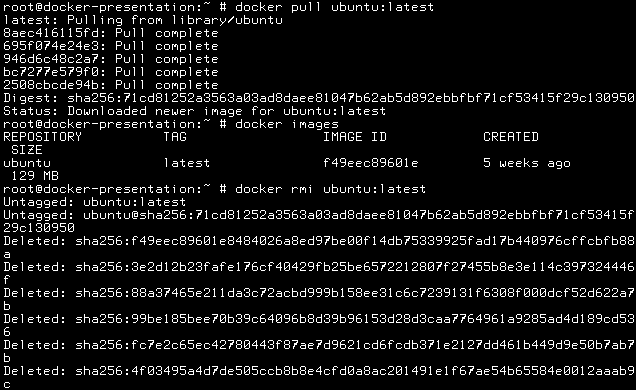
\includegraphics[scale=0.48]{image_1}
\end{frame}

\begin{frame}
  \frametitle{Dockerfile}

  The presupplied images on Docker Hub are good starting points. But
  you will want to build highly customized images. This is
  accomplished by writing a Dockerfile and running the docker build
  command against it.

  Sample Dockerfile:

  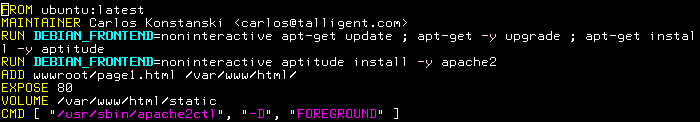
\includegraphics[scale=0.44]{image_3}

  And here is a simple wrapper script to call the docker build command:

  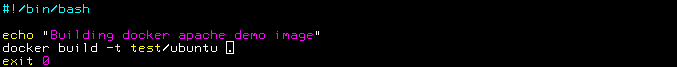
\includegraphics[scale=0.455]{image_4}

  Notice that the build command does not reference Dockerfile, but
  rather the entire current directory. The entire contents of the path
  will get tarred up and passed to the docker container.
\end{frame}

\begin{frame}
  \frametitle{Building}

  Building this sample docker image (lots of output elided):

  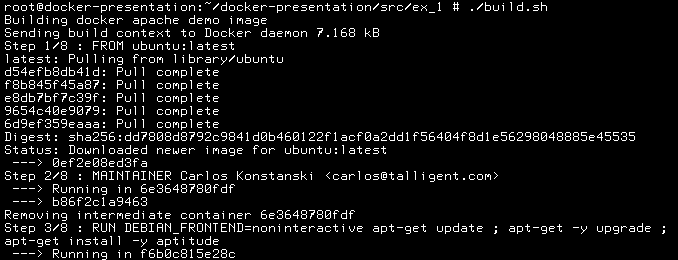
\includegraphics[scale=0.44]{image_2}

  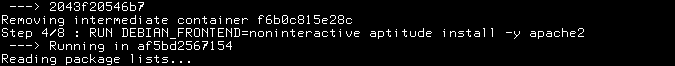
\includegraphics[scale=0.44]{image_5}
\end{frame}

\begin{frame}
  \frametitle{Building}

  Building this sample docker image cont'd:

  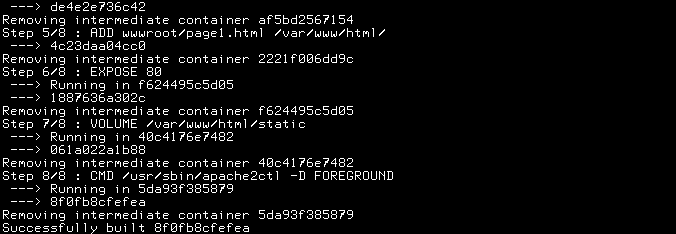
\includegraphics[scale=0.44]{image_6}
\end{frame}

\begin{frame}
  \frametitle{Running}

  The built image and its dependent ubuntu:latest image:

  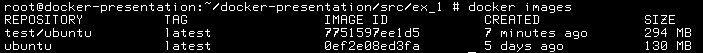
\includegraphics[scale=0.44]{image_7}

  Starting the container:

  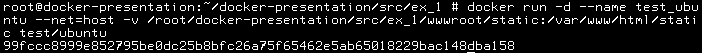
\includegraphics[scale=0.44]{image_8}

  Listing the running container:

  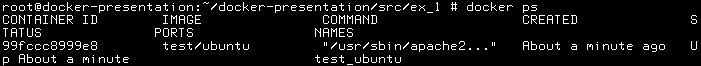
\includegraphics[scale=0.44]{image_9}

  Attaching to the container with a shell and viewing the running
  processes:

  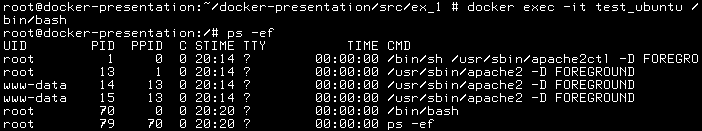
\includegraphics[scale=0.44]{image_10}
\end{frame}

\begin{frame}
  \frametitle{Chroot Filesystem}

  Proof that the container has its own filesystem:

  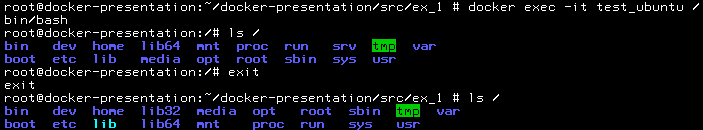
\includegraphics[scale=0.44]{image_11}
\end{frame}

\begin{frame}
  \frametitle{Immutable}

  The contents of a container are immutable. Any changes inside the
  container will only persist until it is stopped. The changes live in
  memory only.

  Before:

  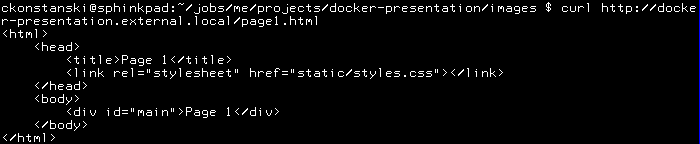
\includegraphics[scale=0.44]{image_12}

  Modify the HTML file:

  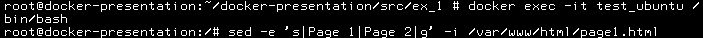
\includegraphics[scale=0.44]{image_14}

  After:

  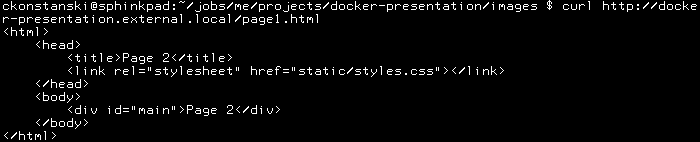
\includegraphics[scale=0.44]{image_13}
\end{frame}

\begin{frame}
  \frametitle{Immutable}

  Stop and restart the container:

  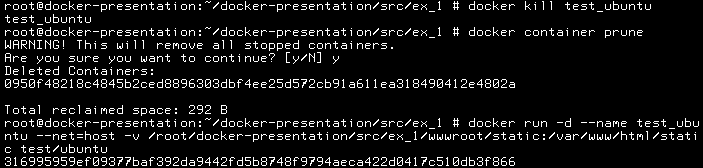
\includegraphics[scale=0.44]{image_15}

  The HTML file is back to its original state:

  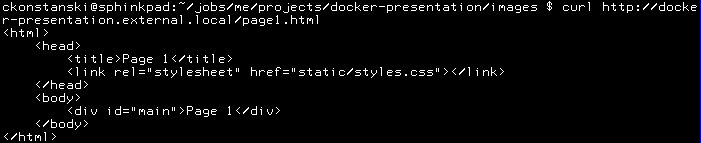
\includegraphics[scale=0.44]{image_16}
\end{frame}

\begin{frame}
  \frametitle{Volumes}

  The way to get filesystem changes to persist is to mount an external
  volume. Our container has such a volume. Recall this line from the
  Dockerfile:

  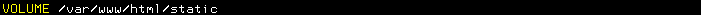
\includegraphics[scale=0.44]{image_17}

  And the -v switch in our run command:

  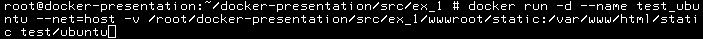
\includegraphics[scale=0.44]{image_18}

  This causes
  /root/docker-presentation/src/ex\textunderscore1/wwwroot/static on
  the host filesystem to be mounted at /var/www/html/static inside the
  container. When processes inside the container modify these files,
  they are actually written to disk on the host filesystem.

  This feature allows the use of containers for databases as one
  obvious example. A database that could not persist its data would be
  useless in most cases. (Occasionally it might actually be a good
  thing.)
\end{frame}

\begin{frame}
  \frametitle{Volumes}

  There is a stylesheet in this volume. Let's modify it while the
  container is running:

  The stylesheet before modifying:

  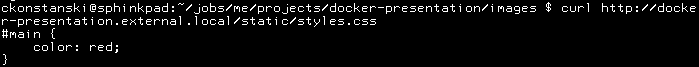
\includegraphics[scale=0.44]{image_19}

  Modify the stylesheet:

  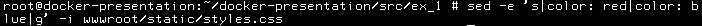
\includegraphics[scale=0.44]{image_20}

  The container sees the change to the stylesheet:

  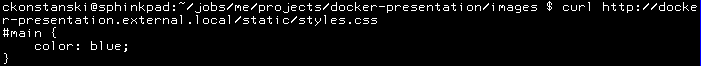
\includegraphics[scale=0.44]{image_21}
\end{frame}

\begin{frame}
  \frametitle{Volumes}

  Restart the container:

  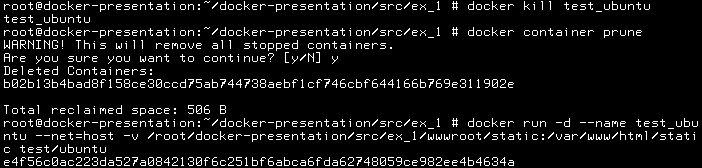
\includegraphics[scale=0.44]{image_22}

  The stylesheet still contains the change:

  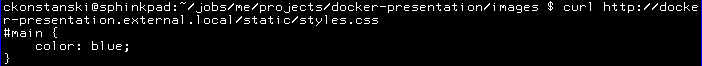
\includegraphics[scale=0.44]{image_23}
\end{frame}

\begin{frame}
  \frametitle{Networking}

  The docker daemon creates a private subnet bridge on the host. The
  gateway of this subnet is the docker0 port.

  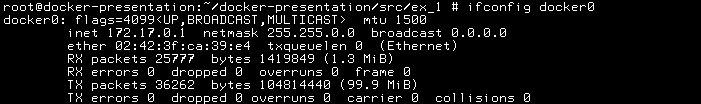
\includegraphics[scale=0.44]{image_24}

  Containers can be run in a variety of networking modes:

  \begin{itemize}
  \item as a node on the docker0 bridge
  \item use a bridge other than the docker0 bridge
  \item attached directly to the host network stack
  \item reuse an existing container's network stack
  \item no networking
  \end{itemize}
\end{frame}

\begin{frame}
  \frametitle{Networking}

  We have been running our container attached directly to the
  host. Notice the --net=host switch in the run command:

  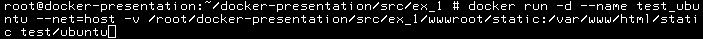
\includegraphics[scale=0.44]{image_18}

  Let's run it attached to the docker0 subnet (default behavior). It
  comes up as 172.17.0.2 on the docker0 bridge:

  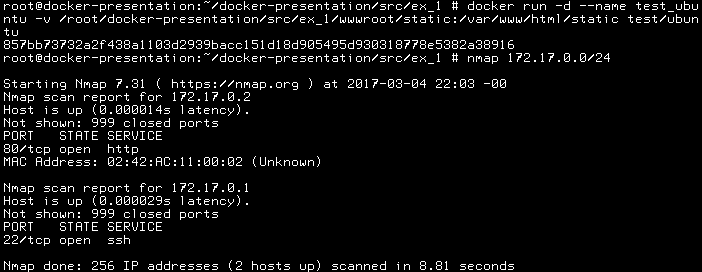
\includegraphics[scale=0.44]{image_25}
\end{frame}

\begin{frame}
  \frametitle{Networking}

  Firewall rules are created automatically by the docker daemon to
  control access to the docker0 bridge.

  FORWARD rules:

  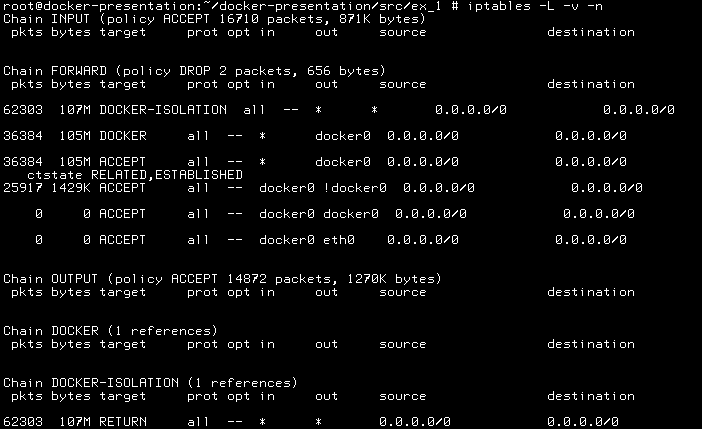
\includegraphics[scale=0.44]{image_26}
\end{frame}

\begin{frame}
  \frametitle{Networking}

  NAT rules:

  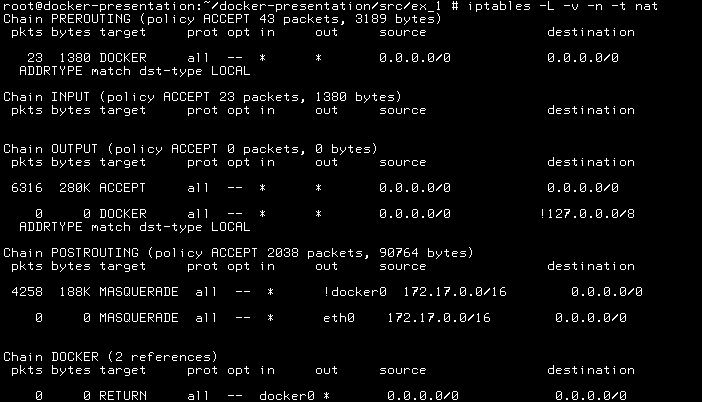
\includegraphics[scale=0.44]{image_27}
\end{frame}

\begin{frame}
  \frametitle{Why Use Docker?}

  By this point you should have a good feel for what docker is. The
  burning question now is: what is docker good for? In this admittedly
  cursory tutorial I have shown you nothing that couldn't be done
  without docker. And I saved this important question for the end when
  usually it would be the opening topic. This is because whenever I
  talk to people about docker without taking the time to first explain
  what docker is, I find it difficult to intelligibly discuss its use
  cases. It's like describing color to a blind person. One has to know
  what docker is first.

  One doesn't choose docker first and then look for reasons to justify
  it. Docker comes into consideration when a problem crops up that
  needs a solution that docker can provide. Even though docker is a
  means to and end and not an end unto itself, there are many reasons
  to use it. Here are just a few that I have personally encountered:
\end{frame}

\begin{frame}
  \frametitle{Why Use Docker?}

  \begin{itemize}
  \item Contain an application's dependencies to avoid fighting with
    packages and configuration installed on the host OS
  \item Run a multi-tier distributed application on one host which
    would otherwise require many hosts
  \item Simplify deployment. One only needs to pull a container. All
    of that messy server configuration can be avoided.
  \item Make it easy to roll back to an earlier version of an
    application without leaving any kruft behind
  \item Use something lighter-weight than a virtual machine. Less
    resource consumption.
  \item Deploy a large and complex application stack very fast because
    it is prebuilt, and in an orchestrated manner (see docker-compose)
  \item Upgrade an application with less downtime
  \end{itemize}

\end{frame}

\end{document}
